
\documentclass[journal]{journal}
\usepackage{csvsimple}
%\usepackage{pgfplotstable}
\usepackage{fancyhdr}

\ifCLASSINFOpdf
\usepackage[pdftex]{graphicx}

  % declare the path(s) where your graphic files are
  % \graphicspath{{../pdf/}{../jpeg/}}
  % and their extensions so you won't have to specify these with
  % every instance of \includegraphics
\DeclareGraphicsExtensions{.pdf,.jpeg,.png}
\else
  % or other class option (dvipsone, dvipdf, if not using dvips). graphicx
  % will default to the driver specified in the system graphics.cfg if no
  % driver is specified.
  % \usepackage[dvips]{graphicx}
  % declare the path(s) where your graphic files are
  % \graphicspath{{../eps/}}
  % and their extensions so you won't have to specify these with
  % every instance of \includegraphics
  % \DeclareGraphicsExtensions{.eps}
\fi
% graphicx was written by David Carlisle and Sebastian Rahtz. It is
% required if you want graphics, photos, etc. graphicx.sty is already
% installed on most LaTeX systems. The latest version and documentation can
% be obtained at: 
% http://www.ctan.org/tex-archive/macros/latex/required/graphics/
% Another good source of documentation is "Using Imported Graphics in
% LaTeX2e" by Keith Reckdahl which can be found as epslatex.ps or
% epslatex.pdf at: http://www.ctan.org/tex-archive/info/
%
% latex, and pdflatex in dvi mode, support graphics in encapsulated
% postscript (.eps) format. pdflatex in pdf mode supports graphics
% in .pdf, .jpeg, .png and .mps (metapost) formats. Users should ensure
% that all non-photo figures use a vector format (.eps, .pdf, .mps) and
% not a bitmapped formats (.jpeg, .png). IEEE frowns on bitmapped formats
% which can result in "jaggedy"/blurry rendering of lines and letters as
% well as large increases in file sizes.
%
% You can find documentation about the pdfTeX application at:
% http://www.tug.org/applications/pdftex






% *** MATH PACKAGES ***
%
\usepackage[cmex10]{amsmath}
% A popular package from the American Mathematical Society that provides
% many useful and powerful commands for dealing with mathematics. If using
% it, be sure to load this package with the cmex10 option to ensure that
% only type 1 fonts will utilized at all point sizes. Without this option,
% it is possible that some math symbols, particularly those within
% footnotes, will be rendered in bitmap form which will result in a
% document that can not be IEEE Xplore compliant!
%
% Also, note that the amsmath package sets \interdisplaylinepenalty to 10000
% thus preventing page breaks from occurring within multiline equations. Use:
\interdisplaylinepenalty=2500
% after loading amsmath to restore such page breaks as IEEEtran.cls normally
% does. amsmath.sty is already installed on most LaTeX systems. The latest
% version and documentation can be obtained at:
% http://www.ctan.org/tex-archive/macros/latex/required/amslatex/math/





% *** SPECIALIZED LIST PACKAGES ***
%
%\usepackage{algorithmic}
% algorithmic.sty was written by Peter Williams and Rogerio Brito.
% This package provides an algorithmic environment fo describing algorithms.
% You can use the algorithmic environment in-text or within a figure
% environment to provide for a floating algorithm. Do NOT use the algorithm
% floating environment provided by algorithm.sty (by the same authors) or
% algorithm2e.sty (by Christophe Fiorio) as IEEE does not use dedicated
% algorithm float types and packages that provide these will not provide
% correct IEEE style captions. The latest version and documentation of
% algorithmic.sty can be obtained at:
% http://www.ctan.org/tex-archive/macros/latex/contrib/algorithms/
% There is also a support site at:
% http://algorithms.berlios.de/index.html
% Also of interest may be the (relatively newer and more customizable)
% algorithmicx.sty package by Szasz Janos:
% http://www.ctan.org/tex-archive/macros/latex/contrib/algorithmicx/




% *** ALIGNMENT PACKAGES ***
%
\usepackage{array}
% Frank Mittelbach's and David Carlisle's array.sty patches and improves
% the standard LaTeX2e array and tabular environments to provide better
% appearance and additional user controls. As the default LaTeX2e table
% generation code is lacking to the point of almost being broken with
% respect to the quality of the end results, all users are strongly
% advised to use an enhanced (at the very least that provided by array.sty)
% set of table tools. array.sty is already installed on most systems. The
% latest version and documentation can be obtained at:
% http://www.ctan.org/tex-archive/macros/latex/required/tools/


\usepackage{mdwmath}
\usepackage{mdwtab}
% Also highly recommended is Mark Wooding's extremely powerful MDW tools,
% especially mdwmath.sty and mdwtab.sty which are used to format equations
% and tables, respectively. The MDWtools set is already installed on most
% LaTeX systems. The lastest version and documentation is available at:
% http://www.ctan.org/tex-archive/macros/latex/contrib/mdwtools/


% IEEEtran contains the IEEEeqnarray family of commands that can be used to
% generate multiline equations as well as matrices, tables, etc., of high
% quality.


\usepackage{eqparbox}
% Also of notable interest is Scott Pakin's eqparbox package for creating
% (automatically sized) equal width boxes - aka "natural width parboxes".
% Available at:
% http://www.ctan.org/tex-archive/macros/latex/contrib/eqparbox/





% *** SUBFIGURE PACKAGES ***
\usepackage[tight,footnotesize]{subfigure}
% subfigure.sty was written by Steven Douglas Cochran. This package makes it
% easy to put subfigures in your figures. e.g., "Figure 1a and 1b". For IEEE
% work, it is a good idea to load it with the tight package option to reduce
% the amount of white space around the subfigures. subfigure.sty is already
% installed on most LaTeX systems. The latest version and documentation can
% be obtained at:
% http://www.ctan.org/tex-archive/obsolete/macros/latex/contrib/subfigure/
% subfigure.sty has been superceeded by subfig.sty.



%\usepackage[caption=false]{caption}
\usepackage[font=footnotesize]{subfig}
% subfig.sty, also written by Steven Douglas Cochran, is the modern
% replacement for subfigure.sty. However, subfig.sty requires and
% automatically loads Axel Sommerfeldt's caption.sty which will override
% IEEEtran.cls handling of captions and this will result in nonIEEE style
% figure/table captions. To prevent this problem, be sure and preload
% caption.sty with its "caption=false" package option. This is will preserve
% IEEEtran.cls handing of captions. Version 1.3 (2005/06/28) and later 
% (recommended due to many improvements over 1.2) of subfig.sty supports
% the caption=false option directly:
%\usepackage[caption=false,font=footnotesize]{subfig}
%
% The latest version and documentation can be obtained at:
% http://www.ctan.org/tex-archive/macros/latex/contrib/subfig/
% The latest version and documentation of caption.sty can be obtained at:
% http://www.ctan.org/tex-archive/macros/latex/contrib/caption/




% *** FLOAT PACKAGES ***
%
\usepackage{fixltx2e}
% fixltx2e, the successor to the earlier fix2col.sty, was written by
% Frank Mittelbach and David Carlisle. This package corrects a few problems
% in the LaTeX2e kernel, the most notable of which is that in current
% LaTeX2e releases, the ordering of single and double column floats is not
% guaranteed to be preserved. Thus, an unpatched LaTeX2e can allow a
% single column figure to be placed prior to an earlier double column
% figure. The latest version and documentation can be found at:
% http://www.ctan.org/tex-archive/macros/latex/base/



\usepackage{stfloats}
% stfloats.sty was written by Sigitas Tolusis. This package gives LaTeX2e
% the ability to do double column floats at the bottom of the page as well
% as the top. (e.g., "\begin{figure*}[!b]" is not normally possible in
% LaTeX2e). It also provides a command:
%\fnbelowfloat
% to enable the placement of footnotes below bottom floats (the standard
% LaTeX2e kernel puts them above bottom floats). This is an invasive package
% which rewrites many portions of the LaTeX2e float routines. It may not work
% with other packages that modify the LaTeX2e float routines. The latest
% version and documentation can be obtained at:
% http://www.ctan.org/tex-archive/macros/latex/contrib/sttools/
% Documentation is contained in the stfloats.sty comments as well as in the
% presfull.pdf file. Do not use the stfloats baselinefloat ability as IEEE
% does not allow \baselineskip to stretch. Authors submitting work to the
% IEEE should note that IEEE rarely uses double column equations and
% that authors should try to avoid such use. Do not be tempted to use the
% cuted.sty or midfloat.sty packages (also by Sigitas Tolusis) as IEEE does
% not format its papers in such ways.


%\ifCLASSOPTIONcaptionsoff
%  \usepackage[nomarkers]{endfloat}
% \let\MYoriglatexcaption\caption
% \renewcommand{\caption}[2][\relax]{\MYoriglatexcaption[#2]{#2}}
%\fi
% endfloat.sty was written by James Darrell McCauley and Jeff Goldberg.
% This package may be useful when used in conjunction with IEEEtran.cls'
% captionsoff option. Some IEEE journals/societies require that submissions
% have lists of figures/tables at the end of the paper and that
% figures/tables without any captions are placed on a page by themselves at
% the end of the document. If needed, the draftcls IEEEtran class option or
% \CLASSINPUTbaselinestretch interface can be used to increase the line
% spacing as well. Be sure and use the nomarkers option of endfloat to
% prevent endfloat from "marking" where the figures would have been placed
% in the text. The two hack lines of code above are a slight modification of
% that suggested by in the endfloat docs (section 8.3.1) to ensure that
% the full captions always appear in the list of figures/tables - even if
% the user used the short optional argument of \caption[]{}.
% IEEE papers do not typically make use of \caption[]'s optional argument,
% so this should not be an issue. A similar trick can be used to disable
% captions of packages such as subfig.sty that lack options to turn off
% the subcaptions:
% For subfig.sty:
% \let\MYorigsubfloat\subfloat
% \renewcommand{\subfloat}[2][\relax]{\MYorigsubfloat[]{#2}}
% For subfigure.sty:
% \let\MYorigsubfigure\subfigure
% \renewcommand{\subfigure}[2][\relax]{\MYorigsubfigure[]{#2}}
% However, the above trick will not work if both optional arguments of
% the \subfloat/subfig command are used. Furthermore, there needs to be a
% description of each subfigure *somewhere* and endfloat does not add
% subfigure captions to its list of figures. Thus, the best approach is to
% avoid the use of subfigure captions (many IEEE journals avoid them anyway)
% and instead reference/explain all the subfigures within the main caption.
% The latest version of endfloat.sty and its documentation can obtained at:
% http://www.ctan.org/tex-archive/macros/latex/contrib/endfloat/
%
% The IEEEtran \ifCLASSOPTIONcaptionsoff conditional can also be used
% later in the document, say, to conditionally put the References on a 
% page by themselves.





% *** PDF, URL AND HYPERLINK PACKAGES ***
%
%\usepackage{url}
% url.sty was written by Donald Arseneau. It provides better support for
% handling and breaking URLs. url.sty is already installed on most LaTeX
% systems. The latest version can be obtained at:
% http://www.ctan.org/tex-archive/macros/latex/contrib/misc/
% Read the url.sty source comments for usage information. Basically,
% \url{my_url_here}.





% *** Do not adjust lengths that control margins, column widths, etc. ***
% *** Do not use packages that alter fonts (such as pslatex).         ***
% There should be no need to do such things with IEEEtran.cls V1.6 and later.
% (Unless specifically asked to do so by the journal or conference you plan
% to submit to, of course. )


% correct bad hyphenation here
\usepackage[none]{hyphenat}


%\pagestyle{empty}
\usepackage{fancyhdr}
\pagestyle{fancy}
%\fancyhf{} % sets both header and footer to nothing
\renewcommand{\headrulewidth}{0pt}
\renewcommand{\footrulewidth}{0pt}
\chead{World Academy of Science, Engineering and Technology \\ ICACII 2015: International Conference on Affective Computing and Intelligent Interaction, Paris, France, (May 18-19,  2015)}
\lfoot{Computer and Information Engineering 2(5) 2015}


%\IEEEpubid{0000--0000/00\$00.00~\copyright~2007 IEEE}

\begin{document}
%\nocite{*}
%
% paper title
% can use linebreaks \\ within to get better formatting as desired
\title{Laban Movement Analysis using Kinect}

\author{Ran~Bernstein, Tal~Shafir, Rachelle~Tsachor, Karen~Studd,
Assaf~Schuster
\thanks{R. Bernstein and A. Schuster are with the Department of Computer
Science, Technion I.I.T, Haifa, Israel}
\thanks{T. Shafir is with the Graduate School of Creative Arts Therapies,
University of Haifa}
\thanks{R. Tsachor is with the School of Theatre \& Music, The University of
Illinois at Chicago}
\thanks{K. Studd is with the School of Dance, George Mason University}}

\maketitle
%\thispagestyle{empty}
%
%
% author names and IEEE memberships
% note positions of commas and nonbreaking spaces ( ~ ) LaTeX will not break
% a structure at a ~ so this keeps an author's name from being broken across
% two lines.
% use \thanks{} to gain access to the first footnote area
% a separate \thanks must be used for each paragraph as LaTeX2e's \thanks
% was not built to handle multiple paragraphs
%



% note the % following the last \IEEEmembership and also \thanks - 
% these prevent an unwanted space from occurring between the last author name
% and the end of the author line. i.e., if you had this:
% 
% \author{....lastname \thanks{...} \thanks{...} }
%                     ^------------^------------^----Do not want these spaces!
%
% a space would be appended to the last name and could cause every name on that
% line to be shifted left slightly. This is one of those "LaTeX things". For
% instance, "\textbf{A} \textbf{B}" will typeset as "A B" not "AB". To get
% "AB" then you have to do: "\textbf{A}\textbf{B}"
% \thanks is no different in this regard, so shield the last } of each \thanks
% that ends a line with a % and do not let a space in before the next \thanks.
% Spaces after \IEEEmembership other than the last one are OK (and needed) as
% you are supposed to have spaces between the names. For what it is worth,
% this is a minor point as most people would not even notice if the said evil
% space somehow managed to creep in.



% The paper headers
%\markboth{World Academy of Science, Engineering and Technology}{International Science Index, Computer and Information Engineering,~Vol.~2, No.~5, May~2015}
%
%{Shell \MakeLowercase{\textit{et al.}}: Bare Demo of IEEEtran.cls for Journals}
% The only time the second header will appear is for the odd numbered pages
% after the title page when using the twoside option.
% 
% *** Note that you probably will NOT want to include the author's ***
% *** name in the headers of peer review papers.                   ***
% You can use \ifCLASSOPTIONpeerreview for conditional compilation here if
% you desire.




% If you want to put a publisher's ID mark on the page you can do it like
% this:
%\IEEEpubidInternational Science Index, Computer and Information Engineering}
% Remember, if you use this you must call \IEEEpubidadjcol in the second
% column for its text to clear the IEEEpubid mark.



% use for special paper notices
%\IEEEspecialpapernotice{(Invited Paper)}






\begin{abstract}
%\boldmath
Laban Movement Analysis (LMA), developed in the dance community
over the past seventy years, is an effective method for observing, describing, notating, and interpreting human
movement to enhance communication and expression in everyday and professional life.
Many applications that use motion capture data might be significantly
leveraged if the Laban qualities will be recognized automatically.
This paper presents an automated recognition method of Laban qualities from
motion capture skeletal recordings and it is demonstrated on the output of
Microsoft's Kinect V2 sensor.
\end{abstract}
% IEEEtran.cls defaults to using nonbold math in the Abstract.
% This preserves the distinction between vectors and scalars. However,
% if the journal you are submitting to favors bold math in the abstract,
% then you can use LaTeX's standard command \boldmath at the very start
% of the abstract to achieve this. Many IEEE journals frown on math
% in the abstract anyway.

% Note that keywords are not normally used for peerreview papers.
\begin{IEEEkeywords}
Laban Movement Analysis, Kinect, Machine Learning.
\end{IEEEkeywords}






% For peer review papers, you can put extra information on the cover
% page as needed:
% \ifCLASSOPTIONpeerreview
% \begin{center} \bfseries EDICS Category: 3-BBND \end{center}
% \fi
%
% For peerreview papers, this IEEEtran command inserts a page break and
% creates the second title. It will be ignored for other modes.
\IEEEpeerreviewmaketitle



\section{Introduction}
% The very first letter is a 2 line initial drop letter followed
% by the rest of the first word in caps.
% 
% form to use if the first word consists of a single letter:
% \IEEEPARstart{A}{demo} file is ....
% 
% form to use if you need the single drop letter followed by
% normal text (unknown if ever used by IEEE):
% \IEEEPARstart{A}{}demo file is ....
% 
% Some journals put the first two words in caps:
% \IEEEPARstart{T}{his demo} file is ....
% 
% Here we have the typical use of a "T" for an initial drop letter
% and "HIS" in caps to complete the first word.
\IEEEPARstart{L}{MA} is a formal language for motion description first
developed by Rudolf Laban \cite{Laban} and colleagues in the middle of the 20th century.
LMA describes both conscious and unconscious human movement, based on Laban's categories of \textit{Body}, \textit{Effort}, \textit{Shape}, and \textit{Space}. 
LMA has been used in the fields of dance, acting, athletics, physical therapy, and psychology and behavioral science.
LMA helps actors create momentary moods and portray personality traits through
movement. For example, LMA work investigates the \textit{Effort} properties
\textit{Flow}, \textit{Space}, \textit{Time} and \textit{Weight} of all movement and helps actors 
think specifically about why their character might move in a jerky, fast, light and direct manner 
versus a heavy, slow, indirect and uninterrupted manner.
\begin{figure*}[ht]
\centering
%\captionsetup{justification=centering}
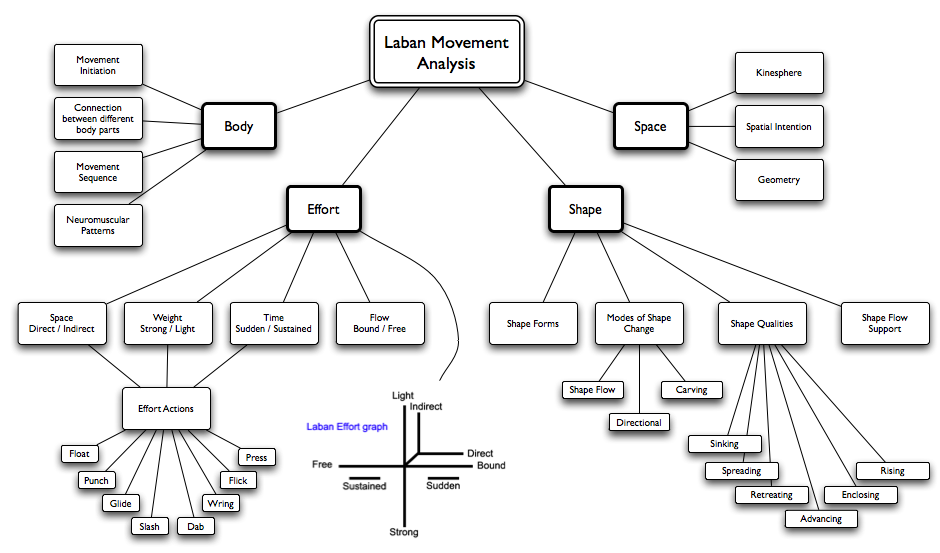
\includegraphics[width=\textwidth]{laban.png}
\caption{Main axes of LMA. Taken from \cite{labanTree}}
\label{labanTree}
\end{figure*}
The entire LMA hierarchy is shown in figure \ref{labanTree}.
\IEEEpubidadjcol

\subsection{Motivation for Automated LMA}
There are numerous applications for computerized identification of the qualities that characterize each possible human movement. Examples include the generation and control of specific expressive movements 
of avatars, virtual characters, or robots in mixed reality scenarios
\cite{Masuda}; detection of personality traits during a job interview
\cite{levy2003use}; early detection, severity assessment or revealing of genetic tendency (phenotype) towards various illnesses such as Alzheimer's,
autism, Parkinson's disease \cite{camurri2003application}, or schizophrenia,
based on analysis of the person's motor behavior. Automated emotion recognition from movement is another 
important application, which may have a variety of uses such as online feedback 
to presenters to help them convey through their body language the emotional message they want to communicate 
(e.g., politicians and public speakers or actors in training) \cite{nguyen2012online}; or recognition 
of people's emotions during interactive games such as those played using the Xbox \cite{Zacharatos}. 
\\\\For reducing our data collection and analysis effort, we focused our work on
18 Laban qualities (as listed in Diagram \ref{oneCMAFinal}) that have been found
predictive for emotional state \cite{ShafirPrivate}.
% needed in second column of first page if using \IEEEpubid
%\IEEEpubidadjcol

\subsection{Related Work}
Several attempts were made to recognize Laban qualities. The first was Chi et al. \cite{chi2000emote}, who quantified \textit{Effort} and \textit{Shape} for animation. Most of the other attempts were for emotion recognition in the context of Human Robot Interaction (HRI). Martin et al. \cite{martin} analyzed the importance of gestures in emotion recognition for HRI. Masuda et al. generated emotional body motion for a human 
form robot \cite{Masuda}. Rett et al. proposed a human motion recognition 
system using a Bayesian reasoning framework \cite{Rett}. The second line of works focused on LMA (not on emotions), but not using Kinect. Lourens et al. \cite{lourens2010communicating} used video data and Samadani et al.
\cite{samadani2013laban} used a high quality MOCAP camera, but both of them
analyzed only hand gestures. A third line of works used Kinect as the main
sensor for skeletal information. Gabel et al.
\cite{gabel2012full} used Kinect for gait analysis. The work of
Zacharatos et al. \cite{Zacharatos} was inspired by LMA for emotion recognition using Kinect. His feature extraction method was influenced by LMA principles, but he did not attempt to recognize the qualities themselves. Kim et al. \cite{kim} did attempt to do so but not on a real dataset and their work did not include a performance evaluation.
\section{Method}
Because we are the first to handle Laban recognition with
Kinect, we had to create a dataset from scratch. To reduce the noise, and ensure that we capture the essence of the Laban qualities in our dataset, we decided that most of it should be built by recording several Certified [Laban] Movement Analysts (CMA), with just a few validation clips taken from recordings of ordinary people. We did not want to constrain the lengths of the clips to be equal, so in order to get feature vectors of uniform length (regardless of the original length of the clips),
every feature is function of a whole clip (for example, the variability of the
elbow's acceleration). On the uniform length feature vector we applied feature
selection, single task learning (learning a model for every quality separately),
and multitask learning (learning a model for all the qualities together).
\subsection{Clip Collection}
Two main datasets were collected: 
\begin{itemize}
  	\item 
	 CMA dataset - includes 6 CMAs performing in about
	80 clips each (a total of 550 clips). Every clip is about 3 seconds long, and the CMAs executed combinations of the 18 qualities. 
	To achieve uniform distribution of the Laban qualities over the dataset, in every 
	clip the CMA was asked to perform actions that include several specific qualities, 
	and nothing but them.
	
	\begin{figure}[h]
	\centering
	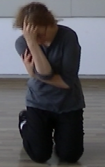
\includegraphics[width=30mm]{Rachelle.png}
	\caption{CMA during a clip}
	\label{Rachelle}
	\end{figure}
	
	\item 
	Non-CMA dataset - includes 2 subjects without a background in movement
	analysis, performing 30 clips each. Every clip is also about 3 seconds long,
	and the subject was asked to perform one out of several
	tasks.
\end{itemize}
\subsection{Clip Labeling}
To achieve a ground truth labeling for the two datasets, every clip was tagged by
a committee of 2 CMAs who determined which Laban qualities appear in the
clip. The use of a committee decision instead of the subjective opinion of one
CMA decreases the labeling noise and the decision is considered as ground truth.
\subsection{Feature Extraction}
Due to unequal length of clips, all the features that were extracted are in
whole clip granularity.
\subsubsection{Primitive Features}
For every joint in the skeleton the angular velocity, acceleration and jerk were
extracted, and for each one of them the mean, variance, skew and kurtosis were
extracted (the extraction of the last four moments is denoted as $\phi$). 
\\\\We denote $\vec{P}_{j}(t)$ as the vector (as we get it from the Kinect) of
the position of joint $j$ in time $t$ in a clip with $n$ frames, and
$\alpha_{j}$ is a coefficient proportional to the mass around the joint.
\subsubsection{Shape Analysis: Sagittal Plane}
Laban shape analysis of the sagittal plane is based on the distinction
between two qualities, \textit{Advance} and \textit{Retreat}. This distinction was quantified by projecting the 
velocity vector of the Center of Mass (CM) on the vector of the front of the
body.
The CM was approximated in this case by the average of all the joints. 
The front of the body was approximated by the perpendicular vector to the vector 
between the Left Shoulder (LS) and
the Right Shoulder (RS).
\\\\If $sag$ stands for sagittal, then from the definition of CM of a physical
system,
\\
\\$\vec{P}_{CM}(t) = \sum_{j \in Joints} \alpha_{j}\vec{P}_{j}(t),
\\
\\\vec{P}_{shoulders}(t)=\vec{P}_{LS}(t)-\vec{P}_{RS}(t),$
\\\\the front is perpendicular to $\vec{P}_{shoulders}$, so we can easily calculate it with:
\\\[\vec{P}_{front}=\vec{P}_{shoulders}\left( \begin{array}{ccc}
0 & 0 & 1 \\
0 & 1 & 0 \\
-1 & 0 & 0 \end{array} \right),\]
\\\\$S_{sag}(t) = \vec{P}_{CM}(t)\cdot\vec{P}_{front}(t),$ 
\\\\$\vec{F}_{sag} = \phi([S_{sag}(1), \ldots S_{sag}(n)]),$
\\\\where $\phi$ was denoted in the beginning of the section.
\subsubsection{Shape Analysis: Horizontal Axis}
Here the distinction is between \textit{Spreading} and \textit{Enclosing} on the horizontal axis.
This distinction was quantified by measuring the average distance between every joint to 
the vertical axis of the body that extends from the Head (H) to the Spine Base (SB).
\\
\\$d_{j} = \frac{\left|(\vec{P}_{j}-\vec{P}_{SB})\times
(\vec{P}_{j}-\vec{P}_{H})\right|}{\left|\vec{P}_{H}-\vec{P}_{SB}\right|},
\\
\\S_{horiz}(t) = \sum_{j \in Joints} d_{j}(t),
\\
\\\vec{F}_{horiz} = \phi([S_{horiz}(1), \ldots S_{horiz}(n)]),$
\subsubsection{Shape Analysis: Vertical Axis}
Here the distinction is between \textit{Rise} and \textit{Sink} on the vertical
axis.
This distinction was quantified by measuring the average distance on axis y of each joint from the CM. This quantification is based on the assumption that the body
is ``longer'' when rising.
\\\\$S_{vert}(t) = \sum_{j \in Joints}
\left|\vec{P}_{j}-\vec{P}_{CM}\right|,
\\\\\vec{F}_{vert} = \phi([S_{vert}(1), \ldots S_{vert}(n)]),$
\subsubsection{LMA Effort Analysis: Time Category}
Here the distinction is between \textit{Sudden} and \textit{Sustained}. This quality was quantified by the skew of the acceleration, relying on the assumption that the
acceleration of a sudden movement will be skewed further to the left, i.e., will get
a higher value at the beginning of the movement.
\subsubsection{Effort Analysis: Space Category}
Here the distinction is between \textit{direct} and \textit{Indirect} motion.
This quality was quantified by the angle between the movement vector of a joint to the next one,
relying on the assumption that in direct movement every vector will be in
the same direction as the last (the angle between them is small).
The velocity direction $V$ is calculated by
$\vec{V}_{j}(t) = \vec{P}_{j}(t+1) - \vec{P}_{j}(t),$
and the angles between a direction to the next one is calculated with the inner product
$\vec{A}_{j}(t) = \vec{V}_{j}(t+1) \cdot \vec{V}_{j}(t).$

\subsection{Performance Evaluation}
From a statistical point of view, we have 18 possible labels (Laban qualities) for every clip. 
Each clip was a combination of just a few of these, often 3-4, which means that there is about 
an 85\% chance that a quality won't appear in a clip. Due to this sparsity, accuracy alone is 
not a relevant metric for the performance evaluation because one can get 85\% accuracy by stating 
that for every recording none of the qualities appear. 
A better evaluation would have to combine the precision and recall rates of the classifier. 
This can be done using the F1 score:
\begin{equation*}
F_{1} = \frac{2\cdot precision\cdot recall}{precision+recall}.
\end{equation*} 
\subsection{Feature Selection}
Every clip is extracted into a vector of 6120 features, most of which are noisy or redundant, thus requiring massive feature selection. The feature selection is done in three stages:
	\begin{itemize}
		\item
		Computing the Anova F-value for every feature over the training set. Cross-validation was used to determine the optimal number of features that should be
		left. As seen in Figure  \ref{selection}, filtering out most of the features yielded better          results than not filtering them, where using the top 4\% of features was optimal.
		\begin{figure}[ht!]
			\centering
			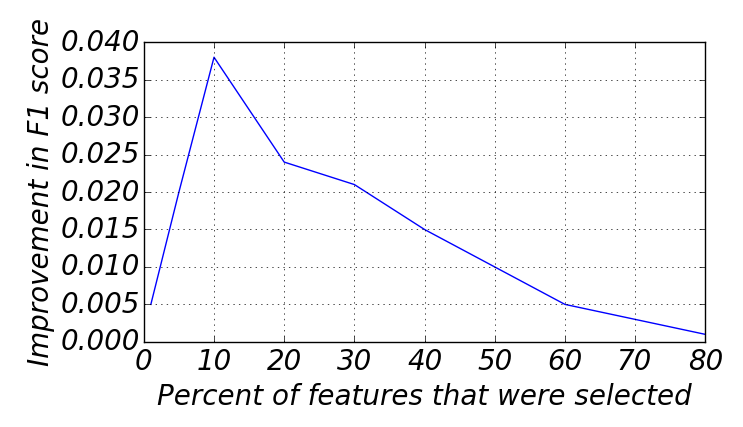
\includegraphics[width=60mm]{featureSelection.png}
			\caption{Influence of the number of features on the performance. The
			selection was made according to statistical significance.
			The blue line is the difference between the score with and without feature
			selection. It can be seen that the optimal fraction of features to select is
			4\%.}
			\label{selection}
			\end{figure}
		\item
			The second phase of feature selection was conducted by Information Gain (IG) rating of the features. As seen in Figure  \ref{igFromFclassif}, the optimal ratio was obtained by selecting the top 60\% out of the features that remained after the first
			phase of feature selection.
			 \begin{figure}[h]
				\centering
				\caption{Influence of the number of features selected with IG from the subset
				of features chosen in the first phase on the performance. The
				optimal ratio was 60\%.}
				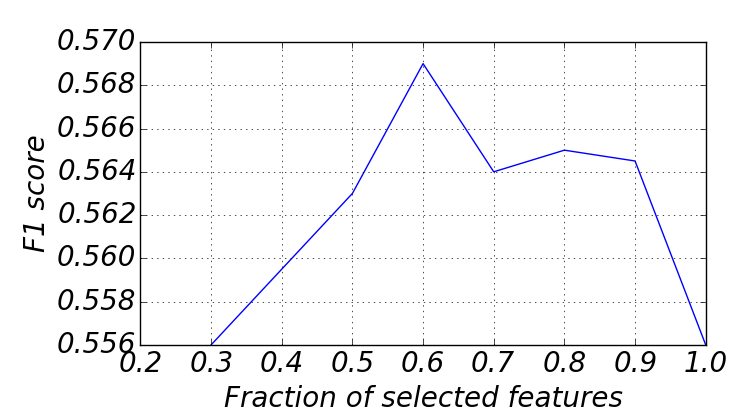
\includegraphics[width=60mm]{igFromFclassif.png}
				\label{igFromFclassif}
			\end{figure}
			Examples of qualities and their most significant feature are given in 
			Table \ref{bestFeatures}. The ``Information Gain'' metric used
			in the table is defined as:
			\begin{equation*}
			       IG(T,f) = H(T) - H(T|f),
			\end{equation*}
			where T is the training set, f is a feature, and H() is the information
			entropy of a dataset.
			
			\begin{table*}[!t]
            \renewcommand{\arraystretch}{1.3}
            \caption{Example of several qualities and the feature found to be
			   the most informative for them. ``Relative position'' stands for the
			   position of the joint relative to the ancestor joint in the joint
			   hierarchy.}
            \label{bestFeatures}
            \centering
            \csvautotabular{rankFeatures.csv}
            \end{table*}
			
		\item
		The third phase of feature section was conducted using the Least Absolute Shrinkage and
		Selection Operator (LASSO) regularization.
	\end{itemize}

\section{Experimental Setups and Results}
\subsection{Multilabel Classification}
Multilabel learning deals with the problem where each instance is associated
with multiple labels simultaneously, where the number of labels is not fixed
from instance to instance. The task of this learning paradigm is to predict
the label (Laban quality) set for each unseen instance (skeletal recording), 
by analyzing training instances with known label sets. The multilabel
approach taken in this paper is to break the LMA problem into 18
binary classification tasks --- one for every Laban quality --- where every binary
decision is whether or not the quality exists.
\\The following subsections will describe several experimental setups
where the results in each will serve as a baseline for the next.
\subsection{Per CMA Evaluation}
	In this experiment the train and test datasets are taken from the same
	CMA. The performance on every Laban quality separately 	is demonstrated on 
	a dataset of one of the CMAs in Figure \ref{oneCMAFinal}.
	In Figure \ref{oneCMASummary} the incremental evolution of the algorithm is 
	described from step to step with the next notation:
	\begin{itemize}
	\item 
	\textit{Chance} stands for randomly tossing a balanced coin in every
	classification decision.
	\item 
	\textit{NN} stands for applying the Nearest Neighbors algorithm.
	\item 
	\textit{LinearSVC} stands for Support Vector Classifier (SVC) with a linear
	kernel.
	\item 
	\textit{LabelBalancing} stands for giving greater weight to clips that
	contain the quality due to the small fraction of them in the whole
	dataset.
	\item 
	\textit{Lasso}, \textit{SFS} (Statistical Feature Selection), and \textit{InfoGain} 
	(information gain based feature selection) were described in the
	\textit{Feature Selection} section.
	\end{itemize}

%\pgfplotstableread{
%x         y    y-max  y-min
%Chance          0.23 0.005 0.005
%NN              0.26 0.025 0.025
%LinearSVC       0.37 0.02  0.02
%LabelBalancing  0.41 0.025 0.025
%Lasso           0.44 0.025 0.025
%SFS             0.48 0.045 0.045
%InfoGain        0.53 0.045 0.045
%}{\mytable}
%\begin{figure}[ht]
%\centering   
%\caption{Evaluation of every CMA's dataset separately in the single task learning
%		setting. Each column represents an additional step in the algorithm's evolution.
%		The results are the average F1 score and its standard deviation (STD) between the CMAs.}
%\begin{tikzpicture}
%\begin{axis} [
%    width=5cm,
%    ymin=0.2,
%    ylabel={F1 score},
%    symbolic x coords={Chance,NN,LinearSVC,LabelBalancing,Lasso,SFS,InfoGain},
%    xtick=data,
%    x tick label style={rotate=90,anchor=east}
%]
%\addplot [ybar, fill=blue!50] 
%  plot [error bars/.cd, y dir=both, y explicit]
%  table [y error plus=y-max, y error minus=y-min] {\mytable};
%\end{axis} 
%\end{tikzpicture}
%\label{oneCMASummary}
%\end{figure}

\begin{figure}[h]
\centering
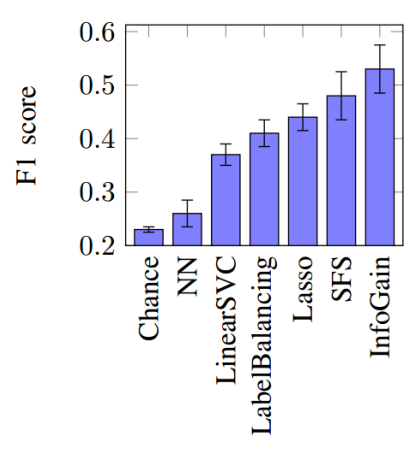
\includegraphics[width=60mm]{Fig5.png}
\caption{Evaluation of every CMA's dataset separately in the single task learning
		setting. Each column represents an additional step in the algorithm's evolution.
		The results are the average F1 score and its standard deviation (STD) between the CMAs.}
\label{oneCMASummary}
\end{figure}
	


\begin{figure*}
	\centering
	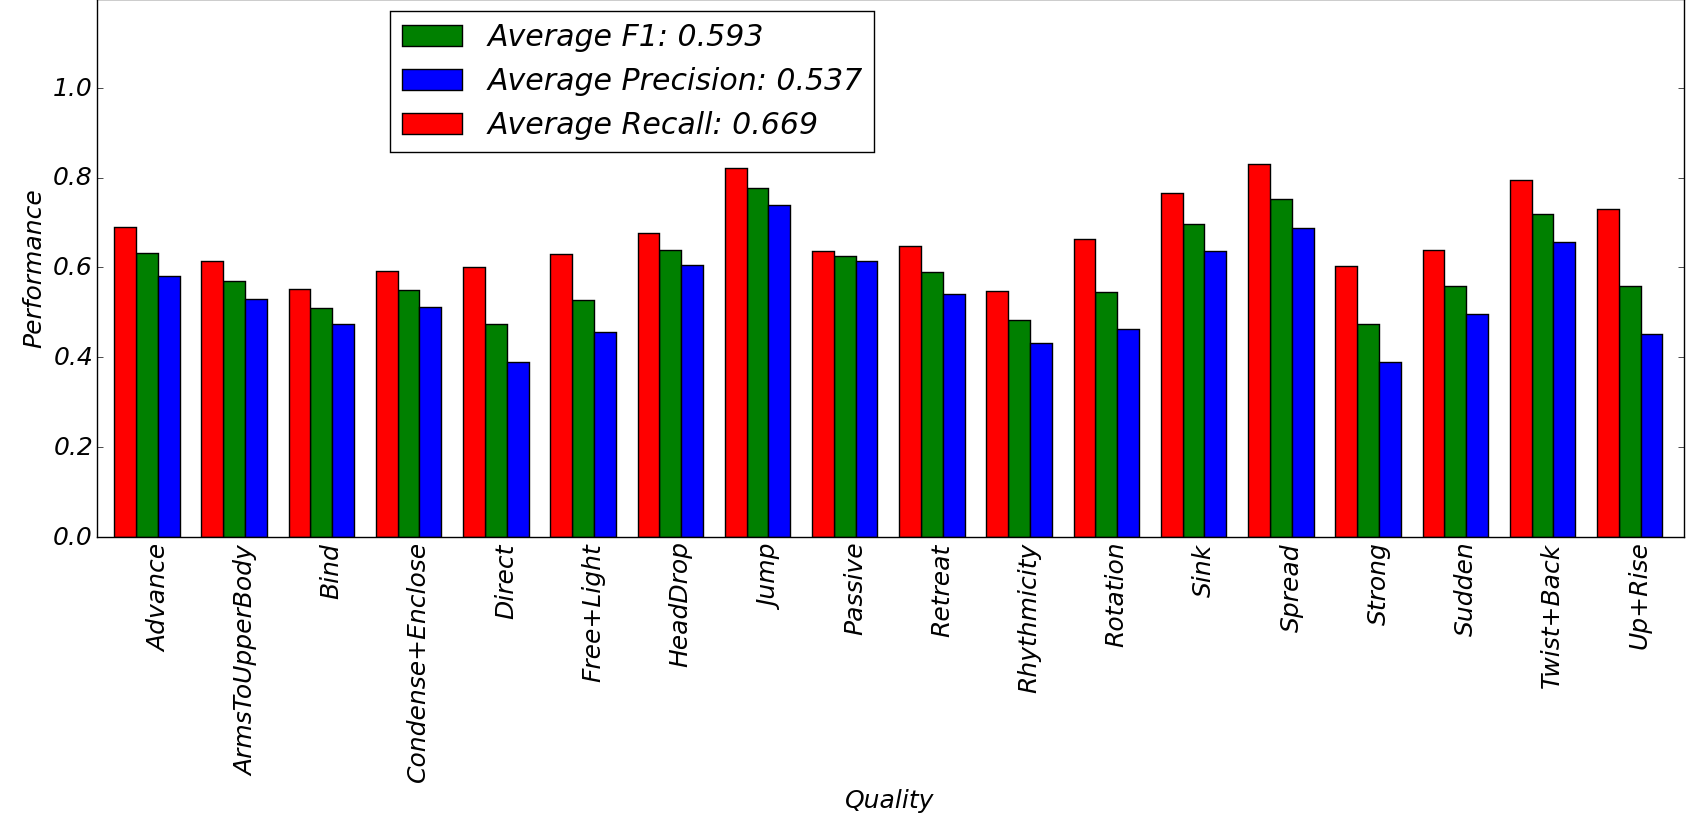
\includegraphics[width=\textwidth, height=60mm]{oneCMAFinalWithoutTitle.png}
	\caption{Recall, precision and F1 score of each Laban quality separately. The
	evaluation was conducted on a dataset that was captured on only one CMA.}
	\label{oneCMAFinal}
\end{figure*}

% An example of a floating figure using the graphicx package.
% Note that \label must occur AFTER (or within) \caption.
% For figures, \caption should occur after the \includegraphics.
% Note that IEEEtran v1.7 and later has special internal code that
% is designed to preserve the operation of \label within \caption
% even when the captionsoff option is in effect. However, because
% of issues like this, it may be the safest practice to put all your
% \label just after \caption rather than within \caption{}.
%
% Reminder: the "draftcls" or "draftclsnofoot", not "draft", class
% option should be used if it is desired that the figures are to be
% displayed while in draft mode.
%
%\begin{figure}[!t]
%\centering
%\includegraphics[width=2.5in]{myfigure}
% where an .eps filename suffix will be assumed under latex, 
% and a .pdf suffix will be assumed for pdflatex; or what has been declared
% via \DeclareGraphicsExtensions.
%\caption{Simulation Results}
%\label{fig_sim}
%\end{figure}

% Note that IEEE typically puts floats only at the top, even when this
% results in a large percentage of a column being occupied by floats.


% An example of a double column floating figure using two subfigures.
% (The subfig.sty package must be loaded for this to work.)
% The subfigure \label commands are set within each subfloat command, the
% \label for the overall figure must come after \caption.
% \hfil must be used as a separator to get equal spacing.
% The subfigure.sty package works much the same way, except \subfigure is
% used instead of \subfloat.
%
%\begin{figure*}[!t]
%\centerline{\subfloat[Case I]\includegraphics[width=2.5in]{subfigcase1}%
%\label{fig_first_case}}
%\hfil
%\subfloat[Case II]{\includegraphics[width=2.5in]{subfigcase2}%
%\label{fig_second_case}}}
%\caption{Simulation results}
%\label{fig_sim}
%\end{figure*}
%
% Note that often IEEE papers with subfigures do not employ subfigure
% captions (using the optional argument to \subfloat), but instead will
% reference/describe all of them (a), (b), etc., within the main caption.


% An example of a floating table. Note that, for IEEE style tables, the 
% \caption command should come BEFORE the table. Table text will default to
% \footnotesize as IEEE normally uses this smaller font for tables.
% The \label must come after \caption as always.
%
%\begin{table}[!t]
%% increase table row spacing, adjust to taste
%\renewcommand{\arraystretch}{1.3}
% if using array.sty, it might be a good idea to tweak the value of
% \extrarowheight as needed to properly center the text within the cells
%\caption{An Example of a Table}
%\label{table_example}
%\centering
%% Some packages, such as MDW tools, offer better commands for making tables
%% than the plain LaTeX2e tabular which is used here.
%\begin{tabular}{|c||c|}
%\hline
%One & Two\\
%\hline
%Three & Four\\
%\hline
%\end{tabular}
%\end{table}


% Note that IEEE does not put floats in the very first column - or typically
% anywhere on the first page for that matter. Also, in-text middle ("here")
% positioning is not used. Most IEEE journals use top floats exclusively.
% Note that, LaTeX2e, unlike IEEE journals, places footnotes above bottom
% floats. This can be corrected via the \fnbelowfloat command of the
% stfloats package.



\section{Conclusion}
We developed a method for recognizing Laban qualities using the Microsoft Kinect
sensor. 
We developed a method for recognizing Laban qualities using the Microsoft
Kinect sensor.
Our method obtained a recall and precision of about 60\% over the qualities.
The larger movements, such as \textit{jump}, \textit{spread}, and \textit{sink},
are easier to quantify, and hence  easier to recognize (precision and recall of 60-90\%).
The more subtle qualities, such as \textit{strong} and \textit{passive},
are harder for us to quantify in kinematic measurements, which causes a degradation in
the performance (precision and recall of 40-60\%).
Overall we believe that we succeeded in capturing the essence of most of the qualities,
using a cheap (\$100) and widely available sensor.
We believe that our work will provide the foundation and inspiration that will make the LMA method
applicable in many more methodologies and processes.




% if have a single appendix:
%\appendix[Proof of the Zonklar Equations]
% or
%\appendix  % for no appendix heading
% do not use \section anymore after \appendix, only \section*
% is possibly needed

% use appendices with more than one appendix
% then use \section to start each appendix
% you must declare a \section before using any
% \subsection or using \label (\appendices by itself
% starts a section numbered zero.)
%



% Can use something like this to put references on a page
% by themselves when using endfloat and the captionsoff option.
\ifCLASSOPTIONcaptionsoff
  \newpage
\fi



% trigger a \newpage just before the given reference
% number - used to balance the columns on the last page
% adjust value as needed - may need to be readjusted if
% the document is modified later
%\IEEEtriggeratref{8}
% The "triggered" command can be changed if desired:
%\IEEEtriggercmd{\enlargethispage{-5in}}

% references section

% can use a bibliography generated by BibTeX as a .bbl file
% BibTeX documentation can be easily obtained at:
% http://www.ctan.org/tex-archive/biblio/bibtex/contrib/doc/
% The IEEEtran BibTeX style support page is at:
% http://www.michaelshell.org/tex/ieeetran/bibtex/
%\bibliographystyle{IEEEtran}
% argument is your BibTeX string definitions and bibliography database(s)
%\bibliography{IEEEabrv,../bib/paper}
%
% <OR> manually copy in the resultant .bbl file
% set second argument of \begin to the number of references
% (used to reserve space for the reference number labels box)
\bibliographystyle{unsrt}
\bibliography{bib}

% biography section
% 
% If you have an EPS/PDF photo (graphicx package needed) extra braces are
% needed around the contents of the optional argument to biography to prevent
% the LaTeX parser from getting confused when it sees the complicated
% \includegraphics command within an optional argument. (You could create
% your own custom macro containing the \includegraphics command to make things
% simpler here.)
%\begin{biography}[{\includegraphics[width=1in,height=1.25in,clip,keepaspectratio]{mshell}}]{Michael Shell}
% or if you just want to reserve a space for a photo:



% You can push biographies down or up by placing
% a \vfill before or after them. The appropriate
% use of \vfill depends on what kind of text is
% on the last page and whether or not the columns
% are being equalized.

%\vfill

% Can be used to pull up biographies so that the bottom of the last one
% is flush with the other column.
%\enlargethispage{-5in}



% that's all folks
\end{document}


